% Fig.3: runtime recording of per-layer start offsets (layer_start
% stack slots) and a bounds-checked field access through them.
% Example: eth/ipv4@outer/udp/gtp/ipv4@inner/tcp where inner.dst == ...
% Build: pdflatex fig_layerstart.tex -> fig_layerstart.pdf
\documentclass[tikz]{standalone}
\usetikzlibrary{positioning, arrows.meta}
\begin{document}
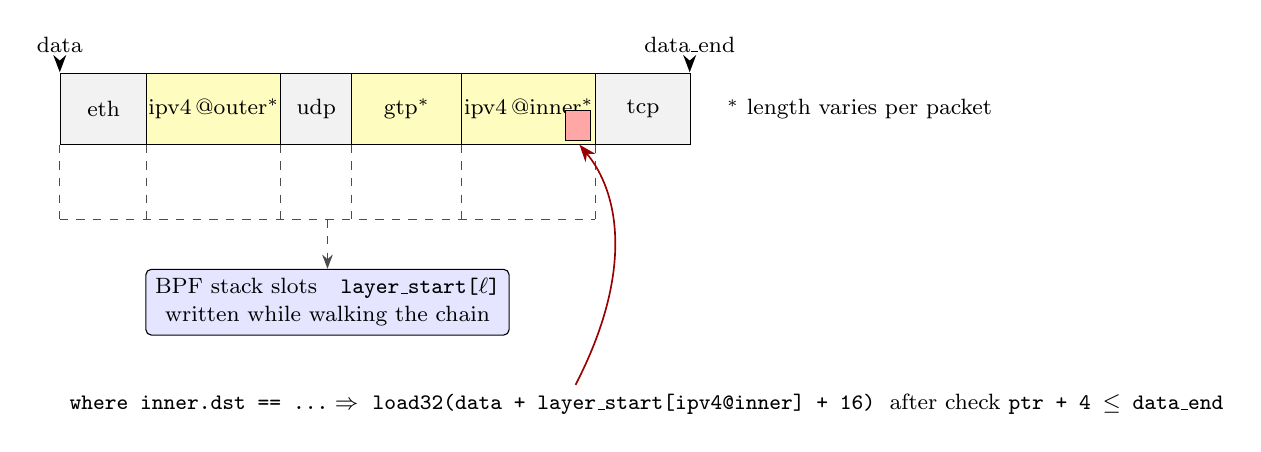
\begin{tikzpicture}[
  font=\small,
  hdr/.style={draw, minimum height=9mm, inner sep=0pt, anchor=south west, align=center},
  fixedhdr/.style={hdr, fill=gray!10},
  varhdr/.style={hdr, fill=yellow!25},
  slot/.style={dashed, gray!60!black},
  arr/.style={-{Stealth[length=2.2mm]}, semithick},
]

% --- packet ribbon (x positions cumulative) ---
\node[fixedhdr, minimum width=11mm] (eth)   at (0,0)      {\footnotesize eth};
\node[varhdr,   minimum width=17mm] (oip)   at (1.1,0)    {\footnotesize ipv4\,@outer$^*$};
\node[fixedhdr, minimum width=9mm]  (udp)   at (2.8,0)    {\footnotesize udp};
\node[varhdr,   minimum width=14mm] (gtp)   at (3.7,0)    {\footnotesize gtp$^*$};
\node[varhdr,   minimum width=17mm] (iip)   at (5.1,0)    {\footnotesize ipv4\,@inner$^*$};
\node[fixedhdr, minimum width=12mm] (tcp)   at (6.8,0)    {\footnotesize tcp};

% highlighted dst field inside inner ipv4 (offset +16, 4 bytes):
% lower strip so the layer label stays readable
\fill[red!35] (6.42,0.05) rectangle ++(0.32,0.38);
\draw (6.42,0.05) rectangle ++(0.32,0.38);

% packet start / data_end markers
\node[font=\footnotesize, anchor=south] at (0,1.05) {data};
\draw[arr] (0,1.0) -- (0,0.92);
\node[font=\footnotesize, anchor=south] at (8.0,1.05) {data\_end};
\draw[arr] (8.0,1.0) -- (8.0,0.92);

% legend for variable-length headers
\node[font=\footnotesize, anchor=west] at (8.35,0.45) {$^*$ length varies per packet};

% --- dashed drops from each layer start onto a bus, then into the stack box ---
\foreach \x in {0, 1.1, 2.8, 3.7, 5.1, 6.8} {
  \draw[slot] (\x,0) -- (\x,-0.95);
}
\draw[slot] (0,-0.95) -- (6.8,-0.95);
\node[draw, rounded corners=2pt, fill=blue!10, minimum height=8mm, align=center]
  (stack) at (3.4,-2.0)
  {\footnotesize BPF stack slots\quad \texttt{layer\_start[$\ell$]}\\[-1pt]
   \footnotesize written while walking the chain};
\draw[slot, -{Stealth[length=1.8mm]}] (3.4,-0.95) -- (stack.north);

% --- example bounds-checked access ---
\node[font=\footnotesize, align=left, anchor=west] (acc) at (0,-3.3)
  {\texttt{where inner.dst == ...}\;$\Rightarrow$\;
   \texttt{load32(data + layer\_start[ipv4@inner] + 16)}\;
   after check \texttt{ptr + 4 $\le$ data\_end}};
\draw[arr, red!60!black] (6.55,-3.05) .. controls (7.3,-1.6) and (7.1,-0.6) .. (6.6,0.0);

\end{tikzpicture}
\end{document}
